\section{CCP4 Refmac protocol}
\label{app:ccp4Refmac}%a060

Protocol designed to refine atomic structures, in reciprocal space, regarding electron density maps in \scipion by using \refmac \citep{vagin2004}, \citep{kovalevskiy2018}. This protocol integrates \refmac functionality in \scipion, supporting accession to \refmac input and output data in the general model building workflow.\\\refmac, Refinement of Macromolecular Structures by the Maximum-Likelihood method, allows the refinement of atomic models against experimental data, and is integrated in CCP4 software suite (\url{www.ccp4.ac.uk/ccp4_projects.php}). Initially applicable to X-ray data, some modifications of \refmac also support optimal fitting of atomic structures into electron density maps obtained from cryo-EM \citep{brown2015}. Particullarly, \refmac considers a five-Gaussian approximation for electron scatttering factors because, unlike of X-rays crystallography, cryo-EM scattering is modified by each atom electric charge and ionization state. In addition, \refmac computes structure factors only for the model-explained part of the map. These structure factors are complex because they include, not only amplitude data, but also phase information. \refmac will try to minimize the difference between the ``observed'' and calculated structure factors, computed from cryo-EM maps and from atom coordinates (structure), respectively. Additional instructions to use \refmac can be found in \url{http://www.ysbl.york.ac.uk/refmac/}.  

\begin{itemize}
  \item Requirements to run this protocol and visualize results:
    \begin{itemize}
        \item \scipion plugin: \ttt{scipion-em-ccp4}
        \item CCP4 software suite (version 7.0.056 or higher)
        \item \scipion plugin: \ttt{scipion-em-chimera}
    \end{itemize}
  \item \scipion menu:
   \ttt{Protocols SPA -> Model building} (\ffigure{fig:app_protocol_refmac_1} (A))
  
  \item Protocol form parameters (\ffigure{fig:app_protocol_refmac_1} (B)):
  
    \begin{figure}[H]
     \centering 
     \captionsetup{width=.7\linewidth} 
     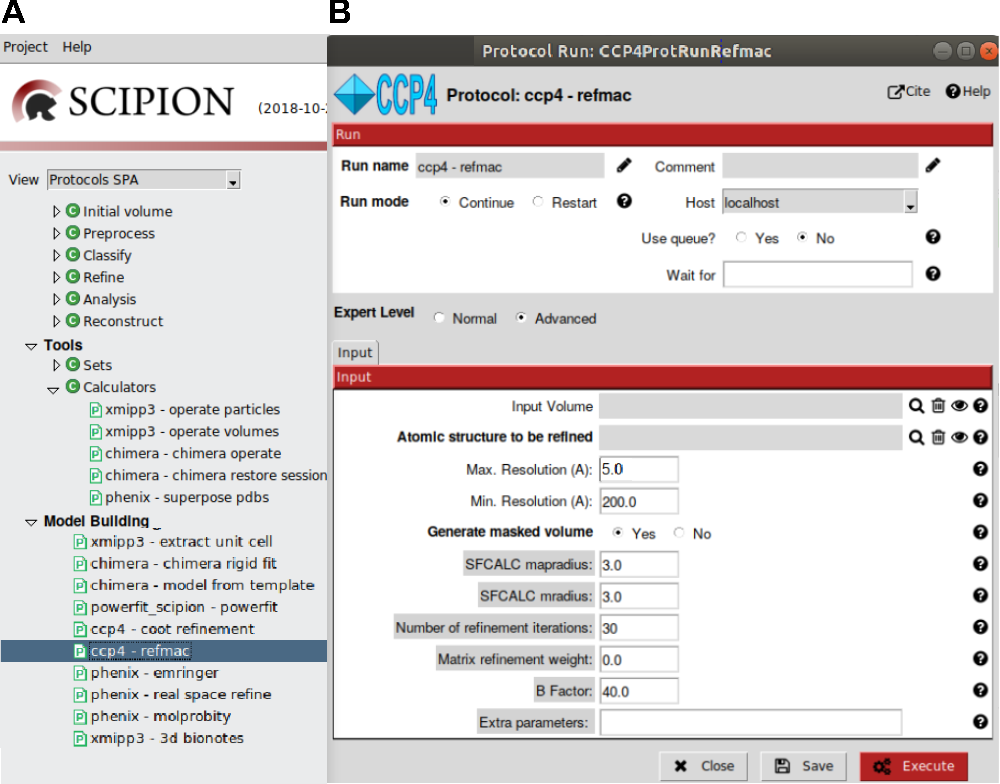
\includegraphics[width=0.90\textwidth]{Images_appendix/Fig126.pdf}
     \caption{Protocol \scommand{ccp4 - refmac}. A: Protocol location in \scipion menu. B: Protocol form.}
     \label{fig:app_protocol_refmac_1}
    \end{figure}

    \begin{itemize}
     \item \ttt{Input Volume/s}: One electron density map previously downloaded or generated in \scipion. An atomic structure should be refined regarding to this volume.
     
     \item \ttt{Atomic structure to be refined}: Atomic structure previously downloaded or generated in \scipion. This structure will be refined according to the electron density volume.
     
     \item \ttt{Max. Resolution (\AA)}: Upper limit of resolution used for refinement, in Angstroms. Using double value of sampling rate is recommendable. 
     
     \item \ttt{Min. Resolution (\AA)}: Lower limit of resolution used for refinement, in Angstroms.
     
     \item \ttt{Generate masked volume}: Parameter set to ``Yes'' by default. With this option, structure factors will be computed for the map around model atomic structure. Otherwise (option ``No''), structure factors will be computed for the whole map.
     
     \item \ttt{SFCALC mapradius}: Advanced parameter that indicates how much around the model atomic structure should be cut. 3\AA\ is the default value.
     
     \item \ttt{SFCALC mradius}: Radius to compute the mask around the model atomic structure. 3\AA\ is the default value.
     
     \item \ttt{Number of refinement iterations}: Cycles of refinement. 30 cycles is the default value.
     
     \item \ttt{Matrix refinement weight}: Weight parameter between electron density map (experimental data) and model atomic structure geometry. Increase this value if you want to give more weight to experimental data. If the value is set to 0.0, bond root mean square deviation from optimal values will be between 0.015 and 0.025.
     
     \item \ttt{B factor}: Geometrical restriction applied to bonded and nonbonded atom pairs. This B factor value set the initial B values.
     
     \item \ttt{Extra parameters}: This parameter gives the opportunity to add some extra \refmac parameters. Use ``$|$'' to separate the next parameter from the previous one.
    \end{itemize}
    
\item Protocol execution:

  Adding specific map/structure label is recommended in \ttt{Run name} section, at the form top. To add the label, open the protocol form, press the pencil symbol at the right side of \ttt{Run name} box, complete the label in the new opened window, press OK and, finally, close the protocol. This label will be shown in the output summary content (see below). If you want to run again this protocol, do not forget to set to \ttt{Restart} the \ttt{Run mode}.\\
  Press the \ttt{Execute} red button at the form bottom.\\
  
  \item Visualization of protocol results:
  
  After executing the protocol, press \ttt{Analyze Results} and a window panel will be opened (\ffigure{fig:app_protocol_refmac_2}). Results can be visualized by selecting each menu element. 
  
  \begin{figure}[H]
     \centering 
     \captionsetup{width=.7\linewidth} 
     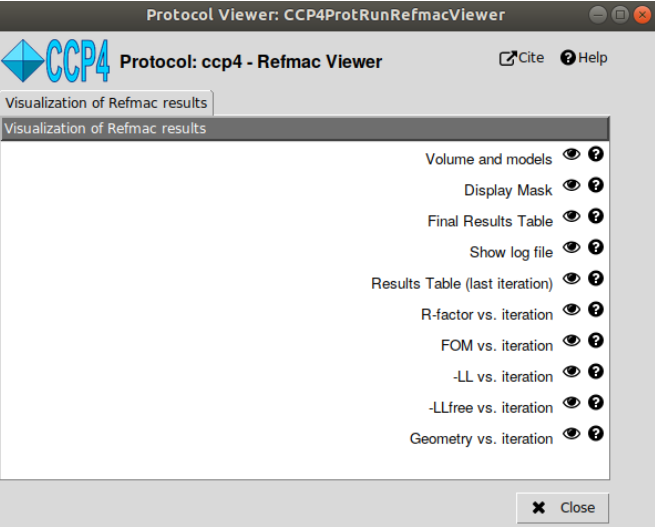
\includegraphics[width=0.60\textwidth]{Images_appendix/Fig127.pdf}
     \caption{Protocol \scommand{ccp4 - refmac}. Menu to visualize \refmac results.}
     \label{fig:app_protocol_refmac_2}
    \end{figure}
    
    Options to visualize \refmac results:
    \begin{itemize}
     \item Volume and models:
     \chimera graphics window displays coordinate axes, selected input volume, starting atomic structure generated by \coot, and final \refmac refined structure (\ffigure{fig:app_protocol_refmac_3}).
        \begin{figure}[H]
         \centering 
         \captionsetup{width=.7\linewidth} 
         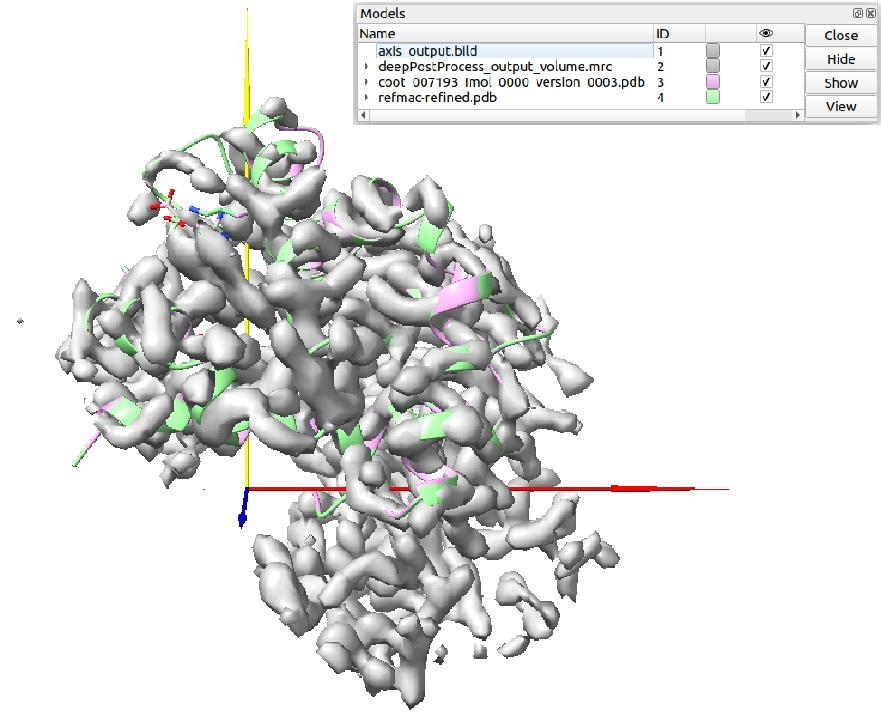
\includegraphics[width=0.80\textwidth]{Images_appendix/Fig128.pdf}
         \caption{Protocol \scommand{ccp4 - refmac}. Map and models visualized with \chimera.}
         \label{fig:app_protocol_refmac_3}
        \end{figure}
     \item Display Mask:
     \chimera graphics window displays the mask generated around the model atomic structure that has to be refined (\ffigure{fig:app_protocol_refmac_4}).
        \begin{figure}[H]
         \centering 
         \captionsetup{width=.7\linewidth} 
         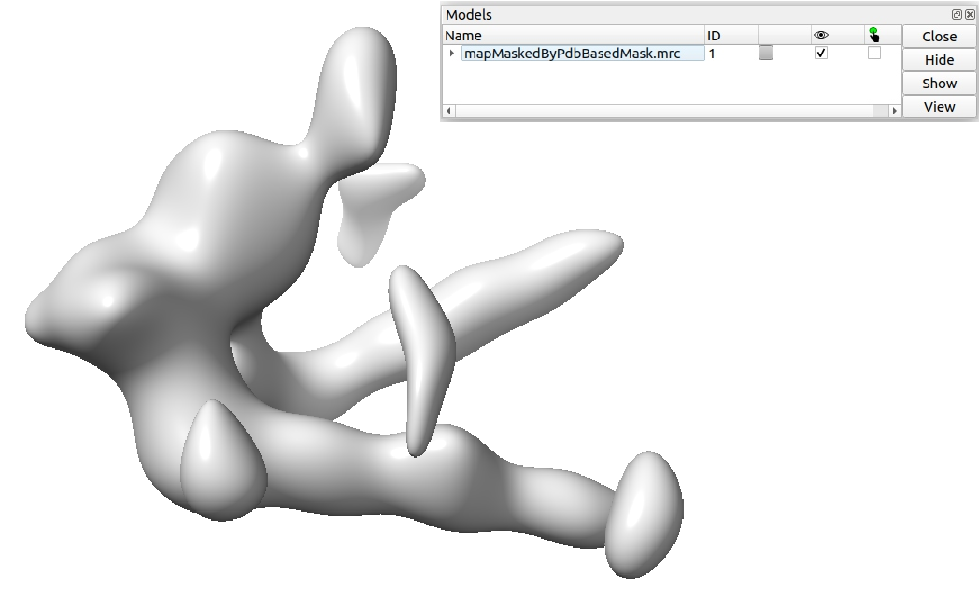
\includegraphics[width=0.80\textwidth]{Images_appendix/Fig129.pdf}
         \caption{Protocol \scommand{ccp4 - refmac}. Mask visualized with \chimera.}
         \label{fig:app_protocol_refmac_4}
        \end{figure}
     \item Final Results Table:
     Table showing the basic statistics of \refmac results. Comparison between initial and final refinement values allows to follow the refinement process. Lower final values than initial ones indicate that discrepancy indices between experimental data and ideal values are disminishing with refinement, which is desirable. R factor and Rms BondLength fair values should be around 0.3 and 0.02, respectively (\ffigure{fig:app_protocol_refmac_5}).
        \begin{figure}[H]
         \centering 
         \captionsetup{width=.7\linewidth} 
         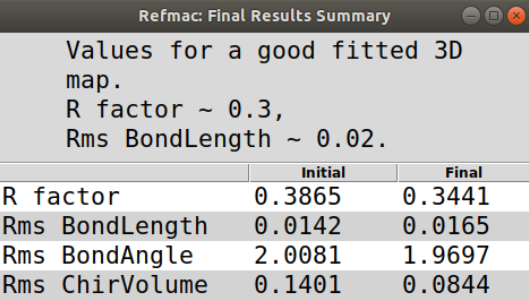
\includegraphics[width=0.40\textwidth]{Images_appendix/Fig130.pdf}
         \caption{Protocol \scommand{ccp4 - refmac}. \refmac final results table.}
         \label{fig:app_protocol_refmac_5}
        \end{figure}
     \item Show log file:
     \refmac-generated text file containing statistics of every \refmac running cycle (\ffigure{fig:app_protocol_refmac_6}).
        \begin{figure}[H]
         \centering 
         \captionsetup{width=.7\linewidth} 
         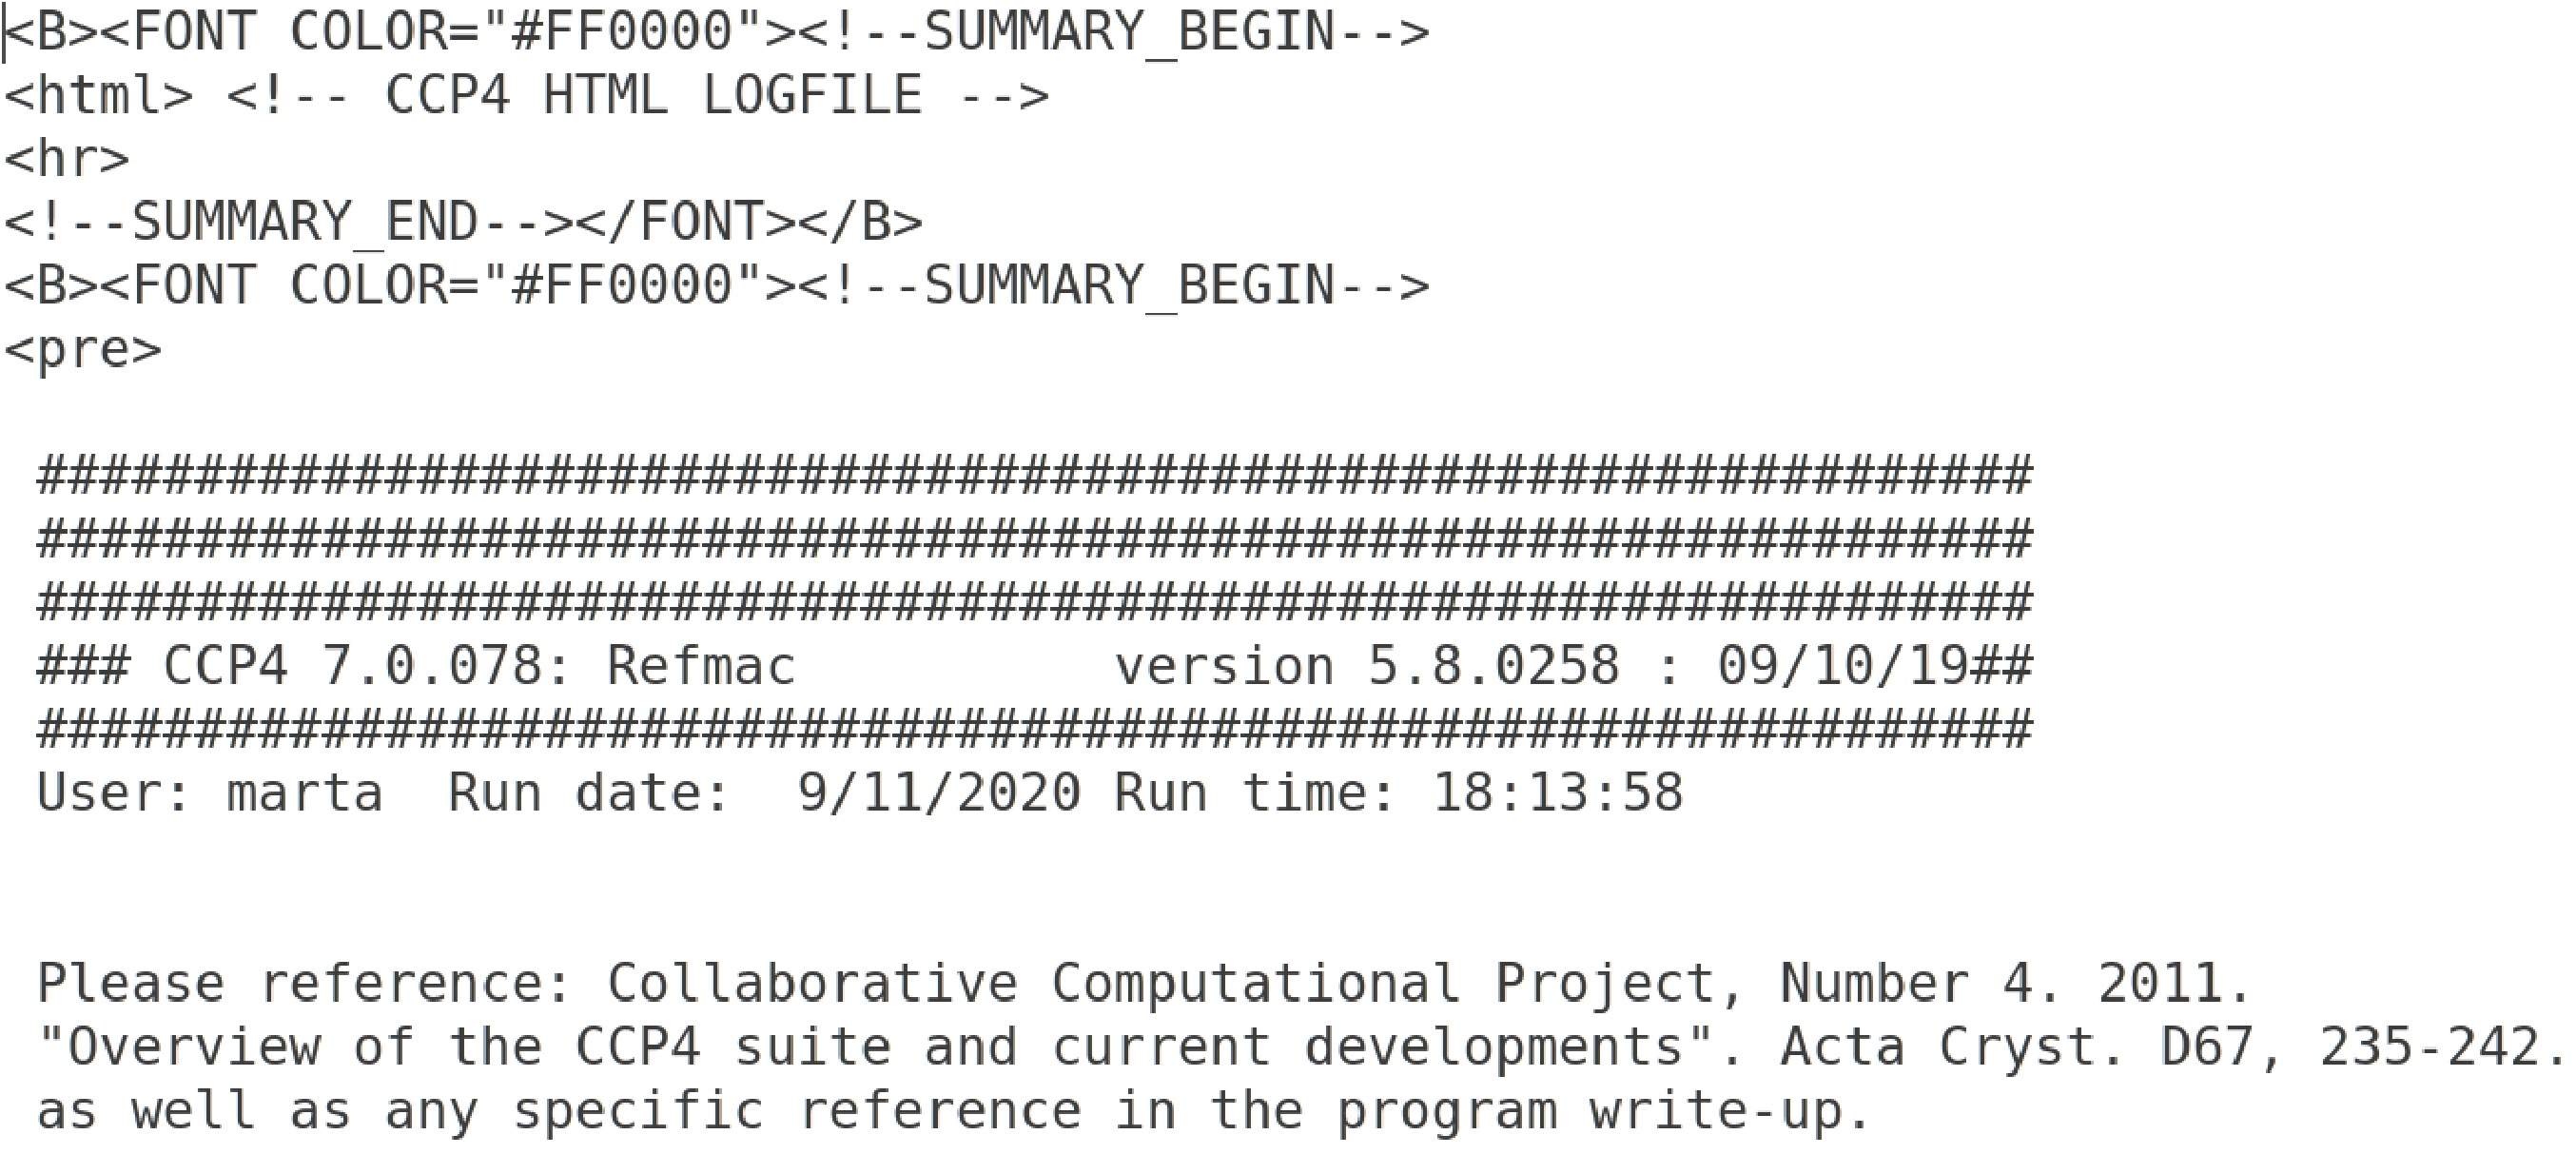
\includegraphics[width=0.80\textwidth]{Images_appendix/Fig131.pdf}
         \caption{Protocol \scommand{ccp4 - refmac}. \refmac raw log file.}
         \label{fig:app_protocol_refmac_6}
        \end{figure}
     \item Results Table (last iteration) (\ffigure{fig:app_protocol_refmac_7}):
        \begin{figure}[H]
         \centering 
         \captionsetup{width=.7\linewidth} 
         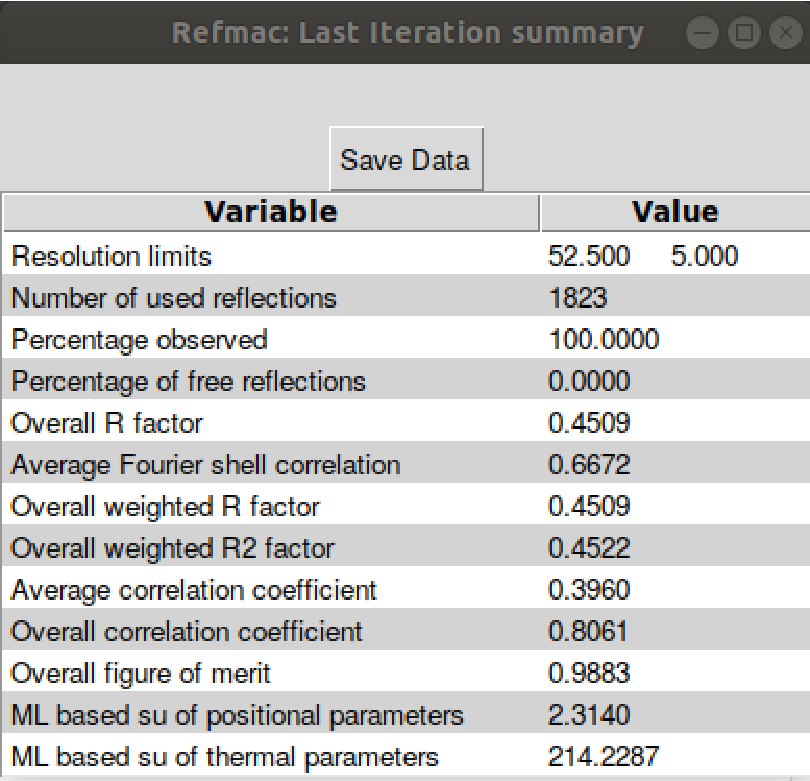
\includegraphics[width=0.60\textwidth]{Images_appendix/Fig132.pdf}
         \caption{Protocol \scommand{ccp4 - refmac}. \refmac last iteration results table.}
         \label{fig:app_protocol_refmac_7}
        \end{figure}
     
     \begin{itemize}
     \item Resolution limits: 0.0 and the resolution value provided as input.
     
     \item Number of used reflections: Each reflection is defined as the common direction that the scattered waves follow, considering all the atoms included in a crystallographic unit cell. A structure factor will be computed for this common direction. The number of reflections is thus identical to the number of structure factors.
     
     \item Percentage observed: Percentage of observed reflections.
     
     \item Percentage of free reflections: Percentage of reflections observed and not included in the refinement process. These reflections are used to compute the \ttt{R factor free}.
     
     \item Overall \ttt{R factor}: Fraction of total differences between observed and computed amplitudes of structure factors, previously scaled, regarding total observed amplitudes of structure factors.\\
     
     \begin{math}
     R factor = \frac{\sum||F_o|-|F_c||}{\sum|F_o|} 
     \end{math}\\
     
     where $|F_o|$ is the observed amplitude of the structure factor and $|F_c|$ is the calculated amplitude of the structure factor.
     
     \item Average Fourier shell correlation: \ttt{FSC}, cross-correlation between shells of two 3D volumes in Fourier space, calculated using complex Fourier coefficients, divided by the number of structure factors in a particular frequency (resolution) shell. \begin{math}FSC_{average}\end{math} has the advantage over \ttt{FSC} of being independent on weight (related with inverse variances of cryo-EM density maps) whenever resolution shells are thin enough that the number of structure factors in each shell is almost equal \citep{brown2015}.
     
     \item Overall weighted \ttt{R factor}: Overall \ttt{R factor} that applies a weight factor to differences between observed and computed amplitudes of structure factors, and also applies that weight factor to the observed amplitudes of structure factors. As in the \begin{math}FSC_{average}\end{math}, the weight is related with inverse variances of cryo-EM density maps.\\
     
     \begin{math}
           weighted R factor = \frac{\sum(w |F_o|-|F_c||)}{\sum(w |F_o|)}
     \end{math}\\
     
     where \ttt{w} is the weight factor.
     
     \item Overall weighted \ttt{R2 factor}: Also known as generalised \ttt{R factor}, this factor is computed as the root square of the fraction of total squares of weighted differences between observed and computed amplitudes of structure factors, previously scaled, regarding the total of weighted squares of observed amplitudes of structure factors.\\
     
     \begin{math}
           weighted R^2 factor = \frac{\sum(w (|F_o|-|F_c||)^2)}{\sum(w (|F_o|)^2)}
     \end{math}\\
     
     \item Average correlation coefficient:
     
     \item Overall correlation coefficient: Correlation between observed and calculated structure factor amplitudes, taking into account only reflections included in the refinement process.
     
     \item Cruickshank's \ttt{DPI} for coordinate error: Diffraction precision index, useful to estimate atomic placement precision. This factor is a function of the number of atoms and reflections included in the refinement, of the overall \ttt{R factor}, of the maximum resolutions of reflections included in the refinement, as well as the completeness of the observed data.
     
     \item Overall figure of merit: $Cosine$ of the error of phases in radians; 1 indicates no error.
     
     \item \ttt{ML} based su of positional parameters: Comprehensive standard uncertainties of positional parameters based on the maximum likelihood function.
     
     \item \ttt{ML} based su of thermal parameters: Comprehensive standard uncertainties of thermal parameters (B values) based on the maximum likelihood function.
     \end{itemize}
     
     \item \ttt{R factor} vs. iteration:
     Plot to visualize \ttt{R factor} and \ttt{R factor free} regarding iterations (\ffigure{fig:app_protocol_refmac_8}):
        \begin{figure}[H]
         \centering 
         \captionsetup{width=.7\linewidth} 
         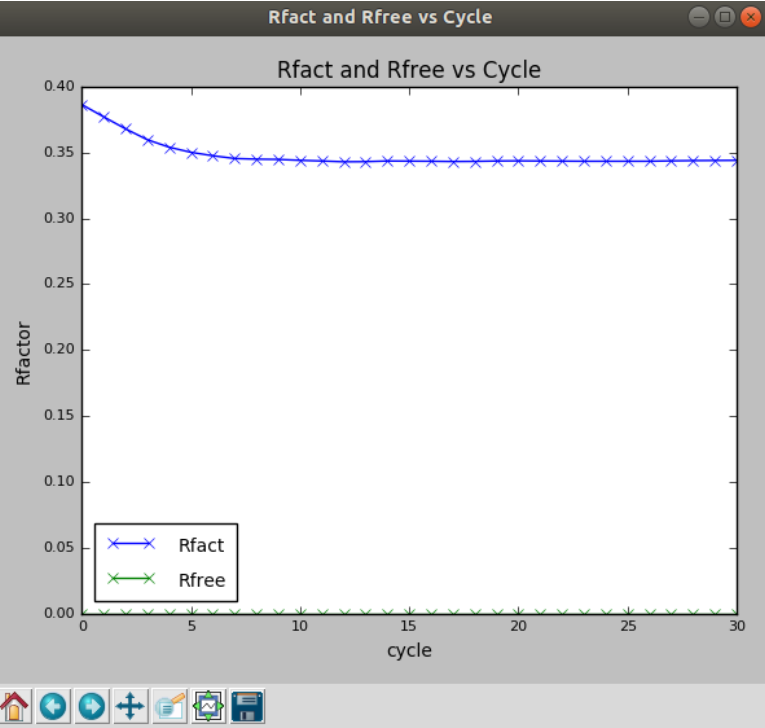
\includegraphics[width=0.60\textwidth]{Images_appendix/Fig133.pdf}
         \caption{Protocol \scommand{ccp4 - refmac}. \ttt{R factor} vs. cycle plot.}
         \label{fig:app_protocol_refmac_8}
        \end{figure}
     \item \ttt{FOM} vs. iteration:
     Plot to visualize Figure Of Merit regarding iterations (\ffigure{fig:app_protocol_refmac_9}):
        \begin{figure}[H]
         \centering 
         \captionsetup{width=.7\linewidth} 
         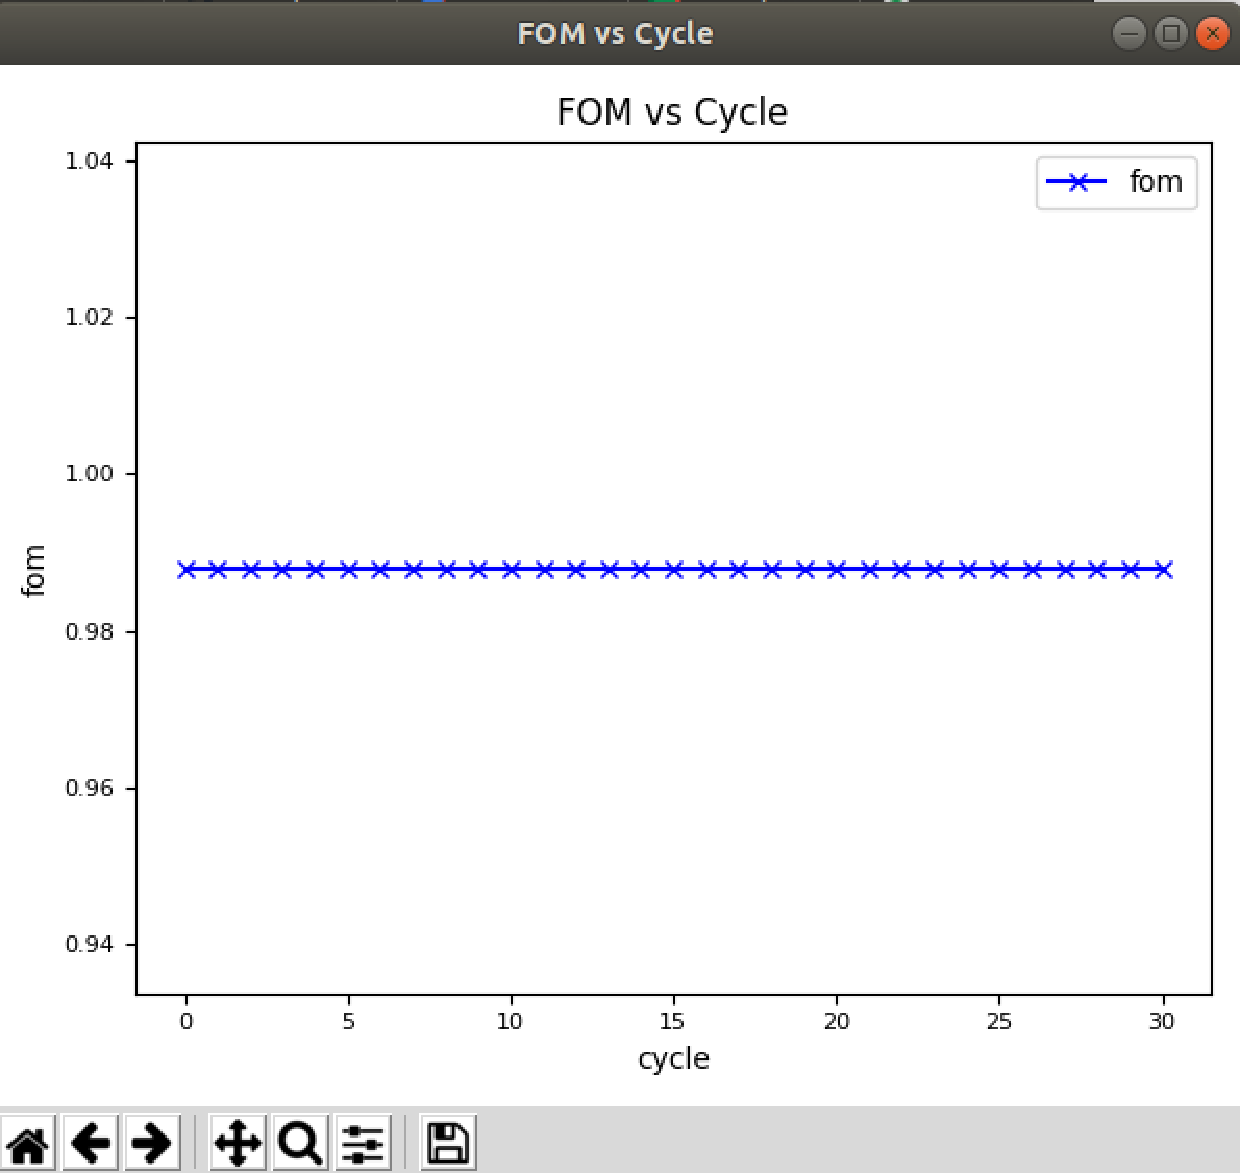
\includegraphics[width=0.60\textwidth]{Images_appendix/Fig134.pdf}
         \caption{Protocol \scommand{ccp4 - refmac}. \ttt{Figure Of Merit} vs. cycle plot.}
         \label{fig:app_protocol_refmac_9}
        \end{figure}
     \item \ttt{-LL} vs. iteration:
     Plot to visualize the log(Likelihood) regarding iterations. Likelihood indicates the probability of a refined model, given the specific observed data  (\ffigure{fig:app_protocol_refmac_10}):
        \begin{figure}[H]
         \centering 
         \captionsetup{width=.7\linewidth} 
         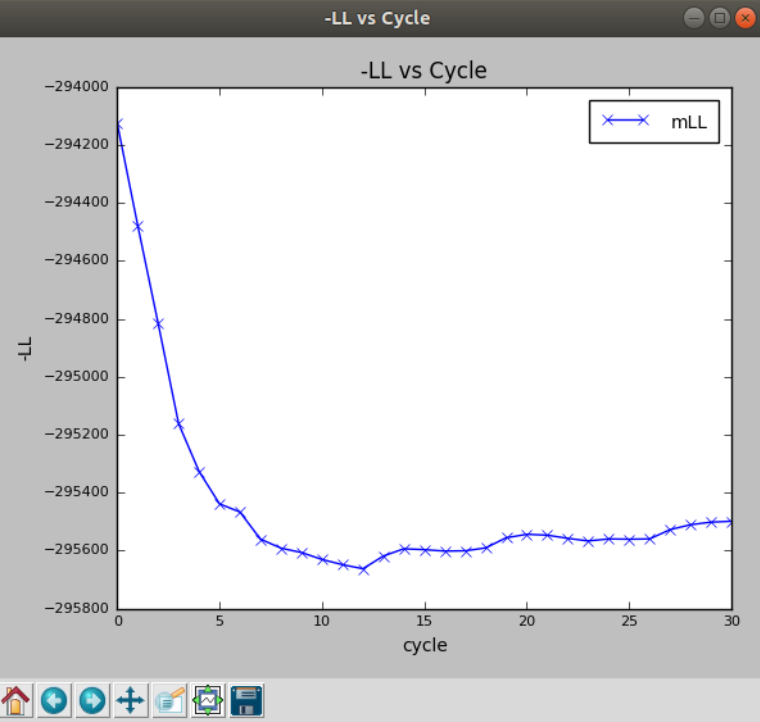
\includegraphics[width=0.60\textwidth]{Images_appendix/Fig135.pdf}
         \caption{Protocol \scommand{ccp4 - refmac}. log(Likelihood) vs. cycle plot.}
         \label{fig:app_protocol_refmac_10}
        \end{figure}
     \item \ttt{-LLfree} vs. iteration:
     Same definition as -LL vs. iteration, although considering only ``free'' reflections not included in refinement
     (\ffigure{fig:app_protocol_refmac_11}):
        \begin{figure}[H]
         \centering 
         \captionsetup{width=.7\linewidth} 
         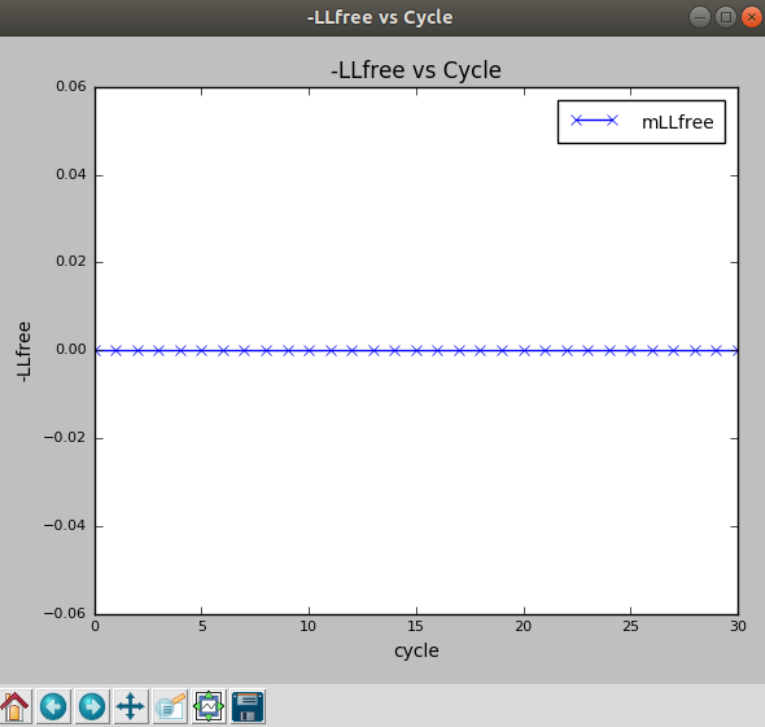
\includegraphics[width=0.60\textwidth]{Images_appendix/Fig136.pdf}
         \caption{Protocol \scommand{ccp4 - refmac}. log(Likelihood) for ``free`` reflections vs. cycle plot.}
         \label{fig:app_protocol_refmac_11}
        \end{figure}
     \item Geometry vs. iteration:
     Plot to visualize geometry parameter statistics regarding iterations (\ffigure{fig:app_protocol_refmac_12}):
     \begin{figure}[H]
         \centering 
         \captionsetup{width=.7\linewidth} 
         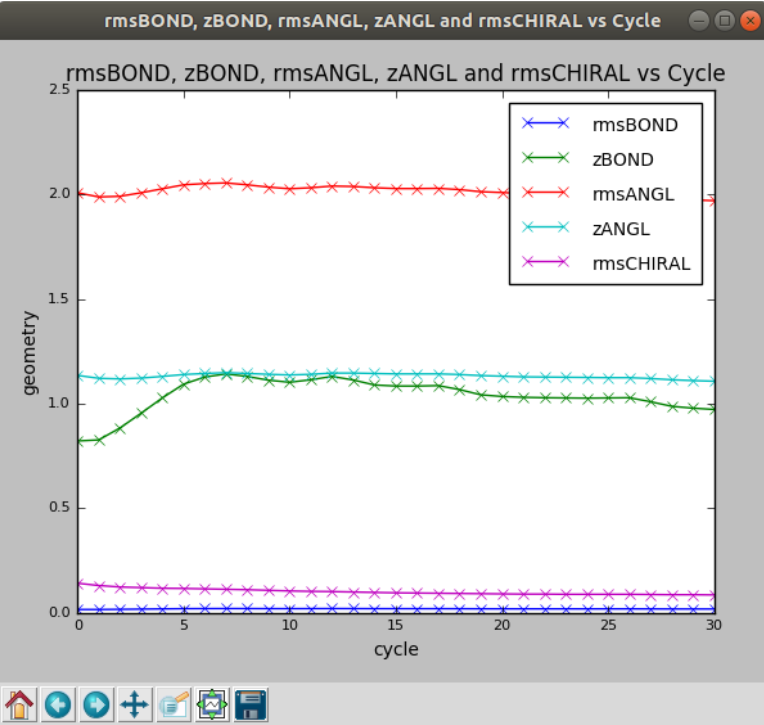
\includegraphics[width=0.60\textwidth]{Images_appendix/Fig137.pdf}
         \caption{Protocol \scommand{ccp4 - refmac}. Geometry parameter statistics vs. cycle plot.}
         \label{fig:app_protocol_refmac_12}
        \end{figure}
     \begin{itemize}
     \item \ttt{rmsBOND}: Root mean square of structure atom covalent bond lengths, computed in \AA, regarding ideal values of bond lengths. Selecting default weighting, \ttt{rmsBOND} values will be around 0.02.
     
     \item \ttt{zBOND}: Number of standard deviations from the mean of covalent bond lengths. Selecting default weighting, \ttt{zBOND} values will be between 0.2 and 1.0.
     
     \item \ttt{rmsANGL}: Root mean square of bond angles from refined structure, computed in degrees, regarding their ideal values. \ttt{rmsANGL} values should converge around 0.1.
     
     \item \ttt{zANGL}: Number of standard deviations from the mean of bond angles. 
     
     \item \ttt{rmsCHIRAL}: Root mean square of chiral volumes from refined structure regarding their ideal values. Chiral volumes are determined by four atoms that form a piramid, and may show positive or negative values. 
     \end{itemize}
    \end{itemize}

 \item Summary content:
  \begin{itemize}
     \item Protocol output (below \scipion framework):\\ \ttt{ccp4 - refmac -> ouputPdb}; \ttt{PdbFile(pseudoatoms=True/ False, volume=True/ False)}.\\Pseudoatoms is set to \ttt{True} when the structure is made of pseudoatoms instead of atoms. Volume is set to \ttt{True} when an electron density map is associated to the atomic structure.
     \item \ttt{SUMMARY} box:\\Statistics included in the above Final Results Table (\ffigure{fig:app_protocol_refmac_13}):
     \begin{figure}[H]
         \centering 
         \captionsetup{width=.7\linewidth} 
         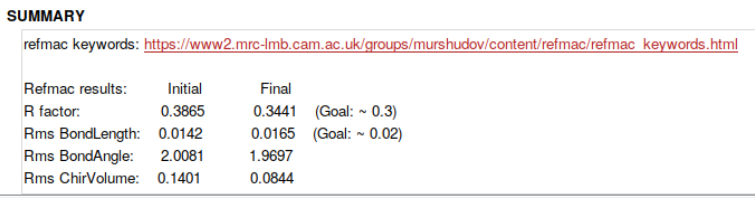
\includegraphics[width=0.80\textwidth]{Images_appendix/Fig138.pdf}
         \caption{Protocol \scommand{ccp4 - refmac}. Summary.}
         \label{fig:app_protocol_refmac_13}
        \end{figure}.\\
    \end{itemize}

  \end{itemize}

    
 %\end{itemize}
